\documentclass[aspectratio=169]{beamer}

\usetheme{Madrid}
\usecolortheme{default}

\usepackage{amsmath, amssymb, mathtools}
\usepackage{booktabs}
\usepackage{hyperref}
\usepackage{graphicx}

\title[GRNG Algorithms (Sec. 2)]{Random Number Generators\\\large Algorithms for Gaussian Samples}
\author{Tanishq Hindoliya}
\institute{Indian Statistical Institute Bangalore}
\date{}

\begin{document}

\begin{frame}
  \titlepage
  \vspace{-0.5em}
  \small
  Based on Section 2 of: D. B. Thomas, W. Luk, P. H. W. Leong, J. D. Villasenor,\
  \textit{Gaussian Random Number Generators}, ACM Computing Surveys (2007).
\end{frame}

\begin{frame}{Scope: Selected Section 2 Methods}
\begin{itemize}
  \item Focus on three generators from Section 2:
  \begin{itemize}
    \item Central Limit Theorem (CLT) sum
    \item Piecewise linear (triangles) approximation
    \item Monty Python packing method
  \end{itemize}
  \item For each: algorithm idea, distribution graph, QQ plot, and complexity.
\end{itemize}
\end{frame}

\begin{frame}{Standard Normal: PDF and CDF}
\small
\begin{block}{Probability density function (PDF)}
\[
\phi(x) = \frac{1}{\sqrt{2\pi}} e^{-x^2/2}.
\]
\end{block}
\begin{block}{Cumulative distribution function (CDF)}
\[
\Phi(x) = \int_{-\infty}^{x} \phi(t)\,dt = \tfrac{1}{2}\Bigl(1 + \mathrm{erf}(x/\sqrt{2})\Bigr).
\]
\end{block}
\begin{itemize}
  \item No closed form for $\Phi$ or $\Phi^{-1}$ \(\Rightarrow\) numerical/approximate evaluation.
\end{itemize}
\end{frame}

\begin{frame}{Approximate vs. Exact (This Talk)}
\begin{columns}[T,onlytextwidth]
\column{0.5\textwidth}
\begin{block}{Approximate methods}
\begin{itemize}
  \item CLT sum (finite $K$)
  \item Piecewise linear triangles
  \item Fast/simple, but tails deviate
\end{itemize}
\end{block}
\column{0.5\textwidth}
\begin{block}{Exact transform}
\begin{itemize}
  \item Monty Python packing
  \item Exact if tail sampler is exact
  \item Fast path dominates most samples
\end{itemize}
\end{block}
\end{columns}
\end{frame}

% --- CLT ---
\begin{frame}{Central Limit Theorem (CLT) Method}
\small
\begin{itemize}
  \item Generate $U_i \sim \mathcal{U}(0,1)$ for $i=1,\dots,K$ and sum $S=\sum U_i$.
  \item Standardize to unit variance:
  \[
  Z=\frac{S-K/2}{\sqrt{K/12}}.
  \]
  \item For $K=12$, $\sqrt{K/12}=1$, so $Z=S-6$ is already $\mathcal{N}(0,1)$-scaled.
  \item Exact for the Irwin--Hall distribution, but only \textbf{approximate} to Gaussian;
  tails are too light for finite $K$.
\end{itemize}
\end{frame}

\begin{frame}{CLT Graph: Histogram vs. Normal}
\centering
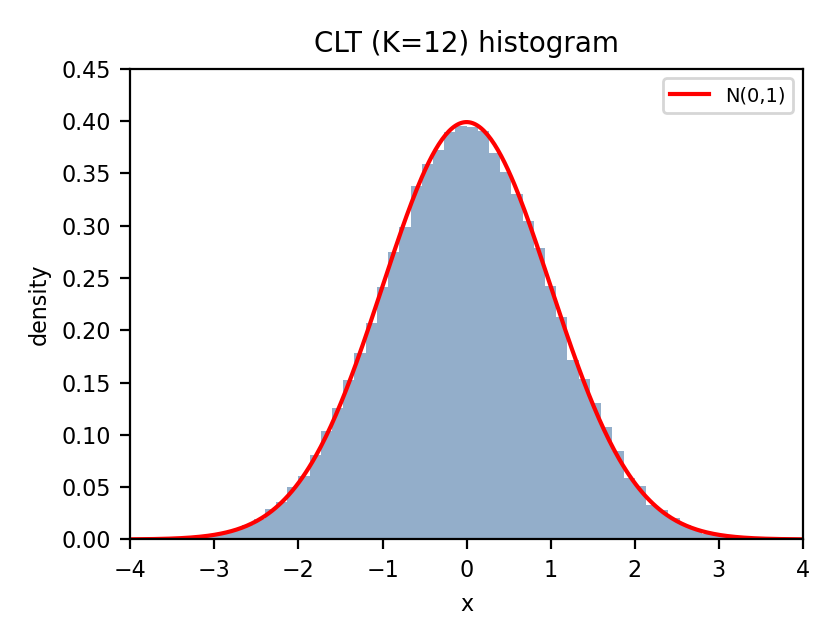
\includegraphics[width=0.80\textwidth,height=0.60\textheight,keepaspectratio]{figures/hist-clt.png}

\vspace{0.3em}
\footnotesize Histogram of CLT samples (K=12) with $\mathcal{N}(0,1)$ overlay; the
center matches well while tails are thin.
\end{frame}

\begin{frame}{QQ Plots: How to Read Them}
\small
\begin{itemize}
  \item X-axis: theoretical quantiles of $\mathcal{N}(0,1)$; Y-axis: sample quantiles.
  \item Points near the 45$^\circ$ line $\Rightarrow$ good distributional match.
  \item Inward bend at extremes $\Rightarrow$ light tails; outward bend $\Rightarrow$ heavy tails.
  \item Kinks/steps suggest piecewise approximations; scatter reflects sampling noise.
\end{itemize}
\end{frame}

\begin{frame}{CLT QQ Plot}
\centering
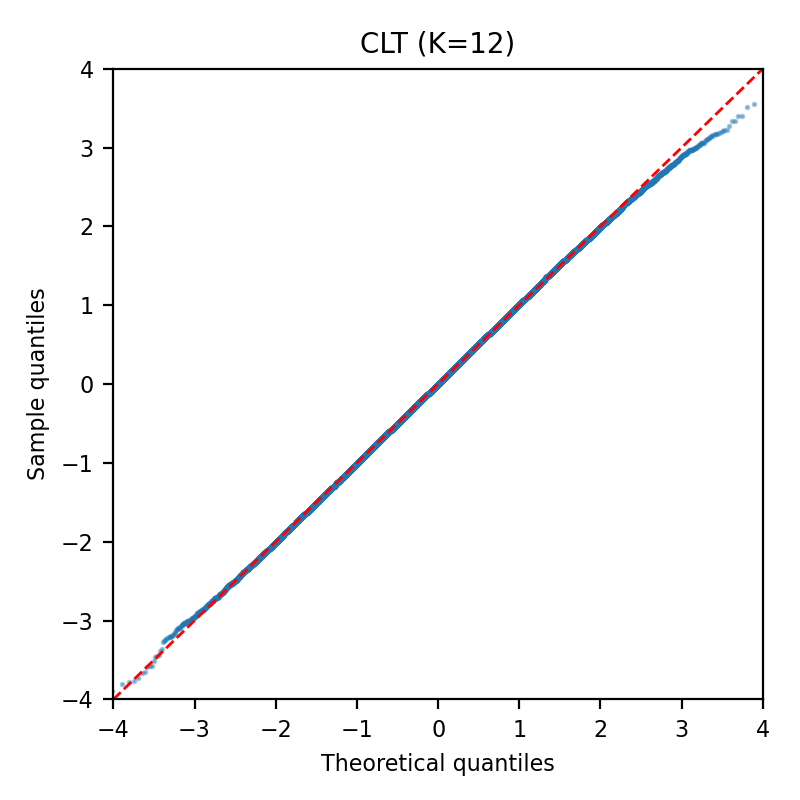
\includegraphics[width=0.70\textwidth,height=0.60\textheight,keepaspectratio]{figures/qq-clt.png}

\vspace{0.3em}
\footnotesize Inward bending in the tails confirms the thin-tail bias of finite $K$ sums.
\end{frame}

% --- Triangles ---
\begin{frame}{Piecewise Linear (Triangles) Method}
\small
\begin{itemize}
  \item Approximate $\phi(x)$ on $[0,x_{\max}]$ by linear segments (triangles), then mirror.
  \item Choose triangle $i$ with probability proportional to its area (alias table).
  \item Sample within the triangle using two uniforms; apply a random sign.
  \item Accuracy improves with more segments and larger $x_{\max}$, but cost grows.
\end{itemize}
\end{frame}

\begin{frame}{Triangles: Basic Idea}
\small
\begin{itemize}
  \item Target: $Z \sim \mathcal{N}(0,1)$ with $\phi(x)=\frac{1}{\sqrt{2\pi}}e^{-x^2/2}$.
  \item Approximate with a mixture of triangular densities:
  \[
  \phi(x)\approx g(x)=\sum_{i=1}^{k} q_i\, t_i(x),
  \]
  \item where $q_i\ge0$ and $\sum_{i=1}^{k} q_i=1$.
\end{itemize}
\end{frame}

\begin{frame}{Triangles: Triangular Component Density}
\small
\[
t_i(x)=
\begin{cases}
\dfrac{1}{w^2}(w-|x-c_i|), & |x-c_i|\le w,\\[6pt]
0, & \text{otherwise}.
\end{cases}
\]
\vspace{0.4em}
\begin{itemize}
  \item Each triangle has width $2w$ and center $c_i$.
  \item Area check: $\frac12(2w)\left(\frac1w\right)=1$.
\end{itemize}
\end{frame}

\begin{frame}{Triangles: Placement and Weights}
\small
\begin{itemize}
  \item Centers equally spaced:
  \[
  c_i=w\left(\frac{k+1}{2}-i\right),\quad i=1,\dots,k.
  \]
  \item Neighboring triangles overlap, yielding a piecewise-linear bell shape.
  \item Weight choice to mimic Gaussian mass:
  \[
  q_i\propto \phi(c_i),\qquad
  q_i=\frac{\phi(c_i)}{\sum_{j=1}^k\phi(c_j)}.
  \]
\end{itemize}
\end{frame}


\begin{frame}{Triangles: Advantages and Limitations}
\small
\begin{columns}[T,onlytextwidth]
\column{0.5\textwidth}
\textbf{Advantages}
\begin{itemize}
  \item Only adds and multiplies.
  \item Hardware-friendly.
  \item Good central accuracy.
\end{itemize}
\column{0.5\textwidth}
\textbf{Limitations}
\begin{itemize}
  \item Approximate, not exact.
  \item Tails less accurate.
  \item More uniforms as $k$ grows.
\end{itemize}
\end{columns}
\end{frame}

\begin{frame}{Triangles Approximation (Fig. 1)}
\centering
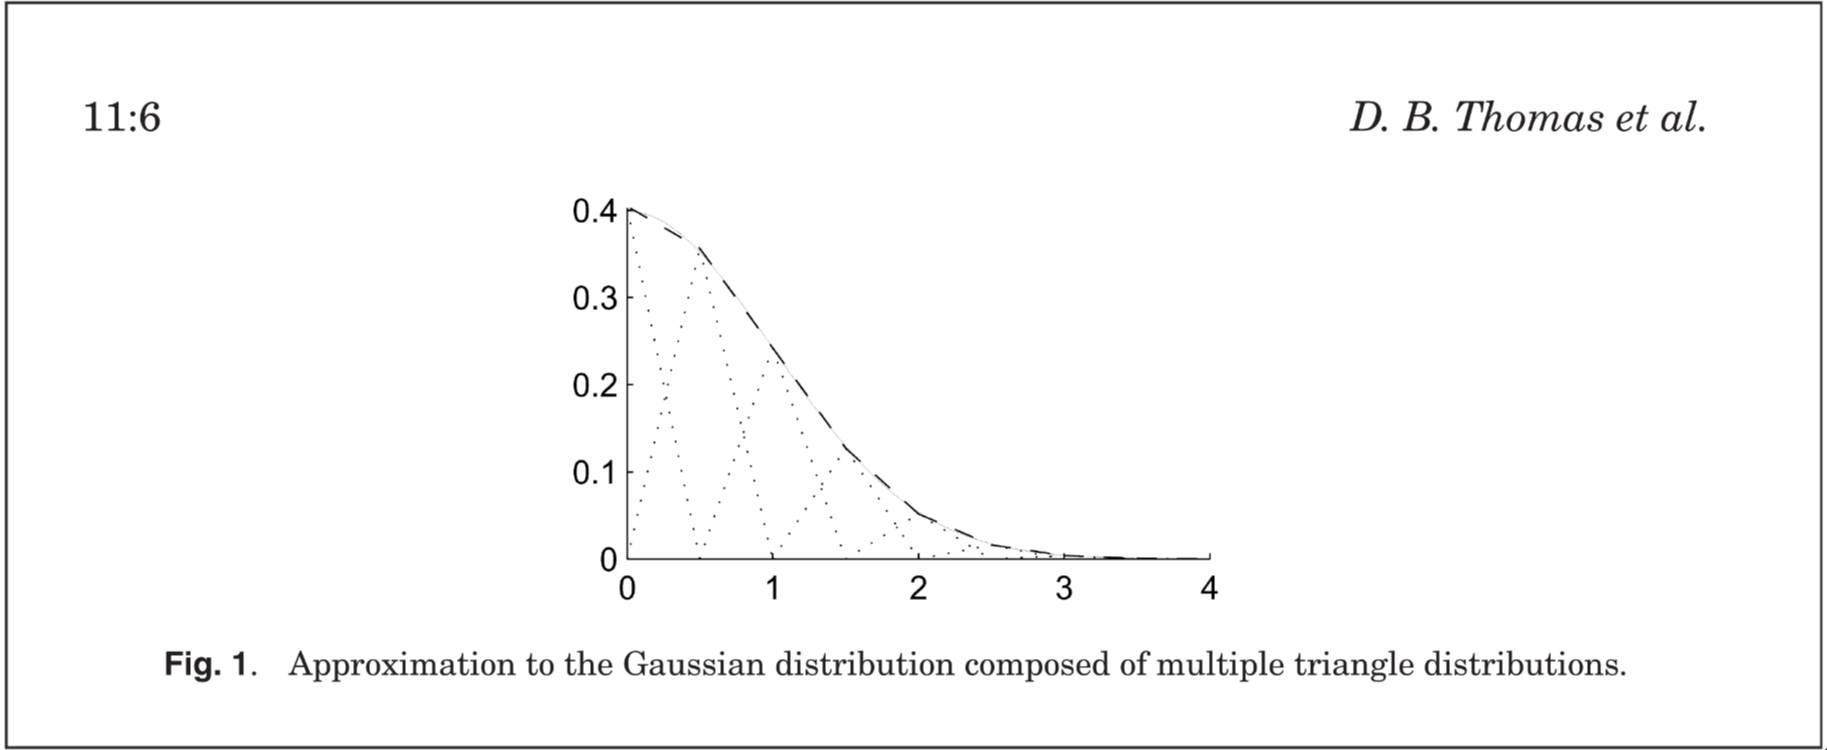
\includegraphics[width=0.92\textwidth,height=0.60\textheight,keepaspectratio]{figures/fig1-triangles.png}

\vspace{0.3em}
\footnotesize Fig. 1 from Thomas et al. (2007): Gaussian approximation using multiple triangle distributions.
\end{frame}

\begin{frame}{Triangles Graph: Histogram vs. Normal}
\centering
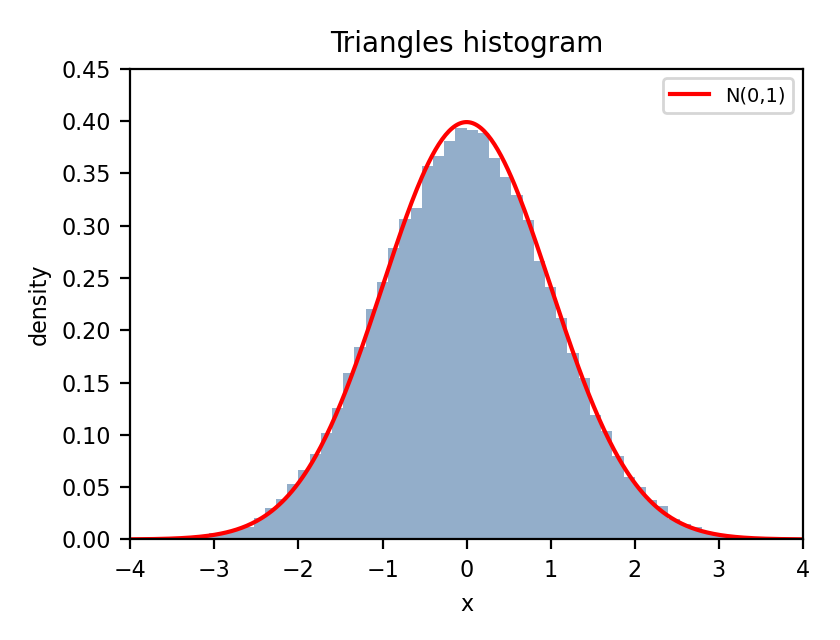
\includegraphics[width=0.80\textwidth,height=0.60\textheight,keepaspectratio]{figures/hist-triangles.png}

\vspace{0.3em}
\footnotesize Histogram shows close central fit with small deviations near the tails and
segment boundaries.
\end{frame}

\begin{frame}{Triangles QQ Plot}
\centering
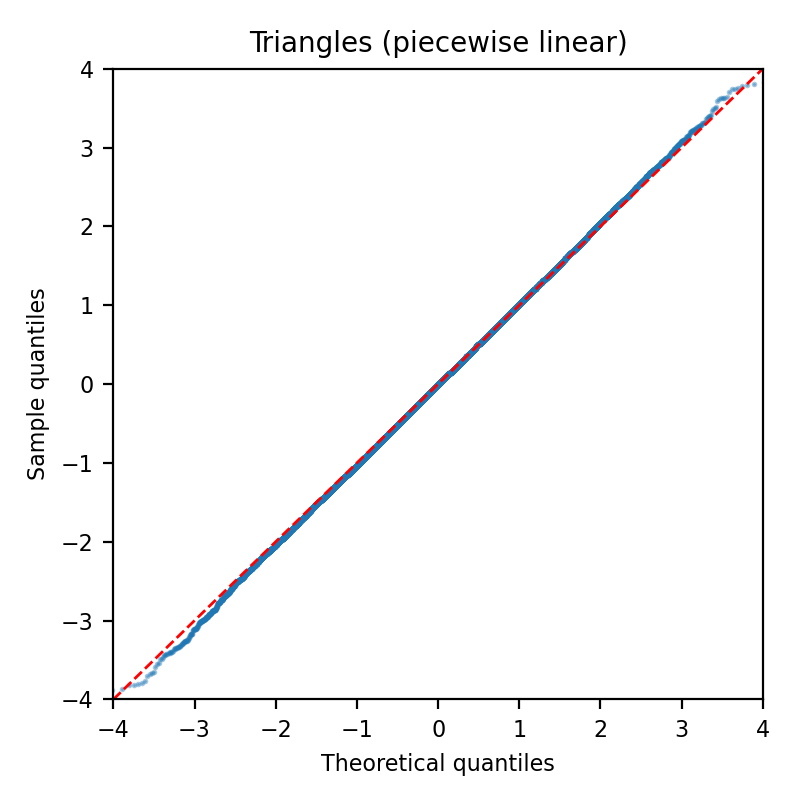
\includegraphics[width=0.80\textwidth,height=0.60\textheight,keepaspectratio]{figures/qq-triangles.png}

\vspace{0.3em}
\footnotesize Small kinks reflect the piecewise-linear approximation; tails deviate from the line.
\end{frame}



% --- Monty Python ---
\begin{frame}{Monty Python Method (Packing)}
\small
\begin{itemize}
  \item Fold the Gaussian PDF into a rectangle of width $b$ and height $1/(2b)$.
  \item Sample a uniform point $(x,y)$ in the rectangle and identify region:
  \begin{itemize}
    \item Areas A/B: return $x$ directly (fast path).
    \item Area C: affine map back; accept if under $\phi(x)$.
    \item Area D: draw from the tail $|x|>b$ with a dedicated tail sampler.
  \end{itemize}
  \item Parameter $b$ trades tail frequency vs overlap (e.g., $b\approx2.29$ gives \(\sim\)2.2\% tail calls).
\end{itemize}
\end{frame}

\begin{frame}{Monty Python: Symmetry Reduction}
\small
\begin{itemize}
  \item Sample the positive half, then attach a random sign.
\end{itemize}
\[
Y=|Z|,\qquad Z=SY,\quad P(S=1)=P(S=-1)=\tfrac12.
\]
\end{frame}

\begin{frame}{Monty Python: Rectangle Construction}
\small
Choose $b>0$ and define:
\[
0\le x\le b,\qquad 0\le y\le \frac{1}{2b}.
\]
Area:
\[
b\cdot\frac{1}{2b}=\frac12.
\]
Sample:
\[
X\sim \mathcal{U}(0,b),\qquad
Y\sim \mathcal{U}\!\left(0,\frac{1}{2b}\right).
\]
\end{frame}

\begin{frame}{Monty Python: Partition into Regions}
\small
Split the rectangle into:
\[
A,\;B,\;C',\;D'.
\]
\begin{itemize}
  \item $A$: always accept ($\phi(x)\ge 1/(2b)$).
  \item $B$: accept if $y<\phi(x)$.
  \item $C'$: affine map into $C$, then re-test.
  \item $D'$: tail region $|x|>b$ handled separately.
\end{itemize}
\end{frame}

\begin{frame}{Monty Python: Region A and B}
\small
Define $a$ by:
\[
\phi(a)=\frac{1}{2b}.
\]
If $x<a$, then $y<\phi(x)$ automatically (accept).
\vspace{0.4em}
Otherwise in $B$, accept if:
\[
y<\phi(x).
\]
\end{frame}

\begin{frame}{Monty Python: Region $C'$ and $D'$}
\small
\begin{itemize}
  \item $C'$: map $(x,y)\mapsto f_C(x,y)$ into $C$; accept if under $\phi(x)$.
  \item The transform preserves area, so probabilities remain correct.
  \item $D'$: corresponds to $|x|>b$; use a separate exact tail sampler.
\end{itemize}
\end{frame}


\begin{frame}{Monty Python: Why It Is Exact}
\small
\begin{enumerate}
  \item Uniform rectangle sampling is exact.
  \item Accepted points under $\phi$ match the Gaussian density.
  \item Area-preserving transforms keep probabilities correct.
  \item Tail sampler is exact.
  \item Random sign restores symmetry.
\end{enumerate}
\end{frame}


\begin{frame}{Monty Python Packing (Fig. 2)}
\centering
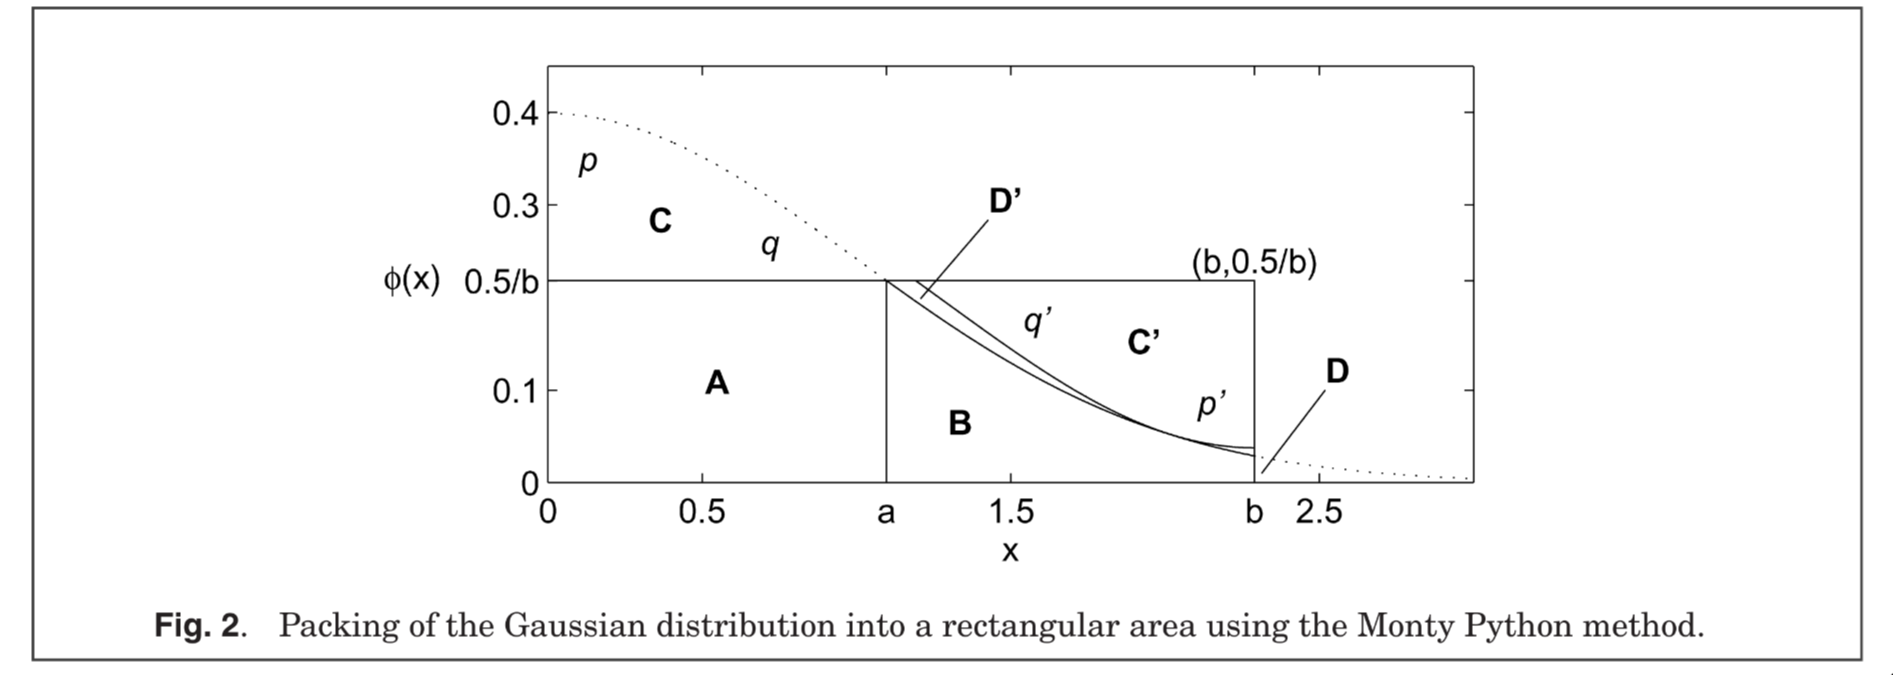
\includegraphics[width=0.92\textwidth,height=0.60\textheight,keepaspectratio]{figures/fig2-monty-packing.png}

\vspace{0.3em}
\footnotesize Fig. 2 from Thomas et al. (2007): Packing of the Gaussian distribution into a rectangle.
\end{frame}

\begin{frame}{Monty Python Graph: Histogram vs. Normal}
\centering
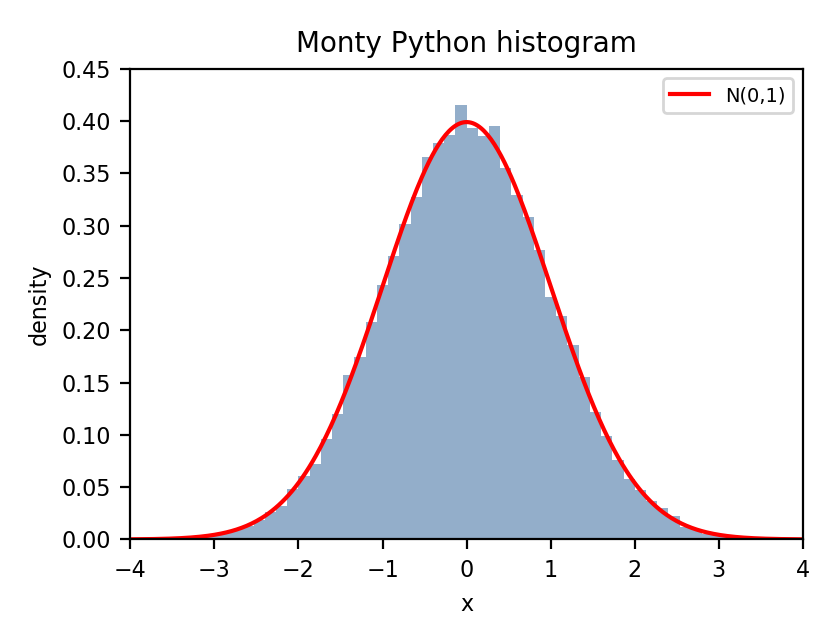
\includegraphics[width=0.80\textwidth,height=0.60\textheight,keepaspectratio]{figures/hist-monty-python.png}

\vspace{0.3em}
\footnotesize Histogram closely matches $\mathcal{N}(0,1)$; differences mostly driven by tail routine.
\end{frame}

\begin{frame}{Monty Python QQ Plot}
\centering
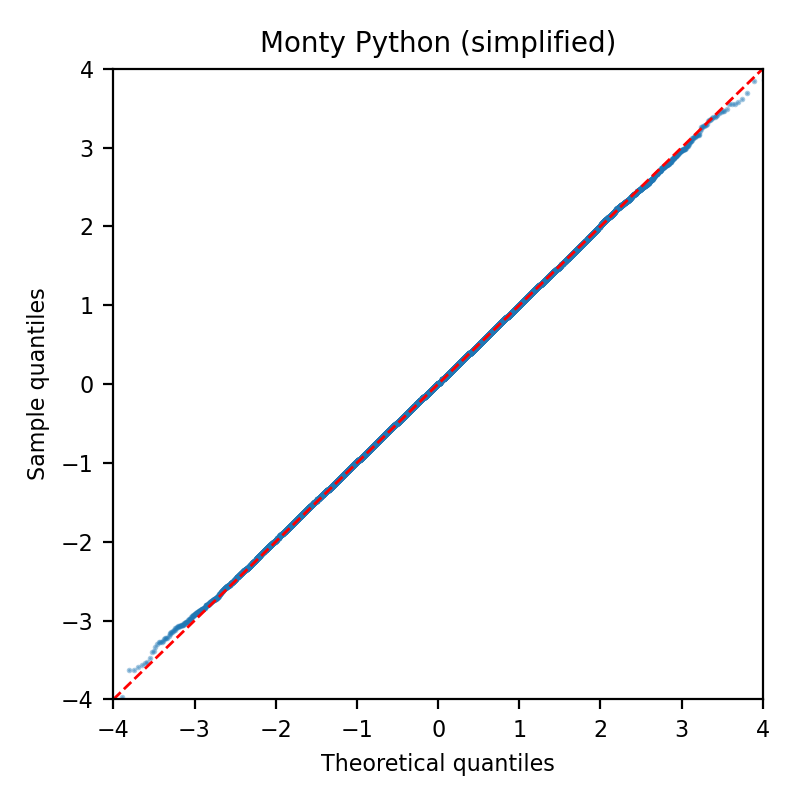
\includegraphics[width=0.80\textwidth,height=0.60\textheight,keepaspectratio]{figures/qq-monty-python.png}

\vspace{0.3em}
\footnotesize Points follow the 45$^\circ$ line across most quantiles, indicating near-exact behavior.
\end{frame}

\begin{frame}{Complexity Comparison}
\scriptsize
\begin{tabular}{@{}p{3.1cm}p{3.6cm}p{6.2cm}@{}}
\toprule
\textbf{Method} & \textbf{Avg cost (uniforms / ops)} & \textbf{Notes} \\
\midrule
CLT sum (K) & $K$ uniforms + $K-1$ adds (O(K)) & Approximate; thin tails unless $K$ is large. \\
Triangles (piecewise) & 2--3 uniforms + alias/table + mult/add & Approximate; quality depends on segments and $x_{\max}$. \\
Monty Python & 2--3 uniforms fast path; occasional $\phi(x)$/tail & Exact if tail sampler exact; efficiency set by $b$. \\
\bottomrule
\end{tabular}
\end{frame}

\begin{frame}{Takeaways}
\small
\begin{itemize}
  \item CLT is simplest but has visibly light tails unless $K$ is large.
  \item Triangles trade accuracy for speed; more segments and larger $x_{\max}$ improve fit.
  \item Monty Python is near-exact with a fast path; performance depends on tail frequency.
\end{itemize}
\end{frame}

\begin{frame}{Reference}
\small
\begin{thebibliography}{9}
\bibitem{thomas2007}
D. B. Thomas, W. Luk, P. H. W. Leong, and J. D. Villasenor.
\newblock \emph{Gaussian Random Number Generators}.
\newblock ACM Computing Surveys, 39(4), Article 11, 2007.\\
\newblock DOI: \href{https://doi.org/10.1145/1287620.1287622}{10.1145/1287620.1287622}.
\end{thebibliography}
\end{frame}
 
\end{document}
